\documentclass[Slovak, a4paper, 12pt]{article}

\usepackage[slovak]{babel}
\usepackage[text={17cm, 24cm}, top=3cm, left = 2cm]{geometry}
\usepackage[T1]{fontenc}
\usepackage[utf8]{inputenc}
\usepackage{times}
\usepackage{graphics}
\usepackage{wrapfig}
\usepackage{rotating}
\usepackage{placeins}

\begin{document}
	\begin{titlepage}
		
		\begin{center}
			\textsc{{\LARGE Vysoké učení technické v Brně \\[0.5em]}  {\LARGE Fakulta informačních technologií}} \\
			\vspace{\stretch{0.382}}
			{\Large Formálne jazyky a prekladače  -- Projekt \\[0.6em]}
			{\huge Prekladač pre jazyk IFJ24} \\[0.6em]
			{\large Tím xluptas00 varianta TRP-izp}
			\vspace{\stretch{0.618}}
			
		\end{center}
		\begin{flushright}
			{ \textbf{Bodové rozdelenie:} 30/25/20/25\% \hfill \textbf{Vedúci: }Samuel Lupták (xluptas00)} \\
			{ \textbf{Implementované rozšírenia:} žiadne\hfill  Petr Němec (xnemecp00)} \\
			{ \hfill  Lukáš Houzar (xhouzal00)} \\
			{\today \hfill Mário Klopan (xklopam00)}
		\end{flushright}
		
	\end{titlepage}
	
	\section{Návrh}
	\noindent Prekladač sa skladá z 3~hlavných častí a 4~pomocných dátových štruktúr.\\
	\textbf{Hlavné časti} prekladača (a ich podčasti):
	\begin{itemize}
		\item Lexikálny analyzátor \footnote[1]{Ďalej len \textit{skener}}
		\item Dvojprechodový syntaktický a sématický analyzátor \footnote[2]{Ďalej len \textit{parser}}
		\begin{itemize} 
			\item Analýza kódu pomocou rekurzívneho zostupu
			\item Analýza výrazov pomocou precedenčnej analýzy
		\end{itemize}
		\item Generátor výsledného kódu
	\end{itemize}
	
	\noindent\textbf{Pomocné štruktúry} použité v prekladači:
		\begin{itemize}
		\item  Tabuľka s rozptýlenými položkami s implicitným zreťazením položiek \footnote[3]{Ďalej len \textit{hašovacia tabulka}}
		\item Abstraktný syntaktický strom \footnote[4]{Ďalej len \textit{ASS}}
		\item Zásobník
		\item Fronta
	\end{itemize}
	
	\noindent \textbf{Využitie} jednotlivých štruktúr je nasledovné:\\
	\par\textit{Hašovacia tabulka: } Bola použitá pre implementáciu tabuľky symbolov. Podmienka pre implicitné zreťazenie nám 
	robila mierny problém, pretože teoreticky nekonečný počet identifikátorov sa nevmestí do konečne veľkej tabuľky \\
	\par\textit{ASS: } Slúži na komunikáciu medzi parserom a generátorom kódu\\
	\par\textit{Zásobník: } Je využitý precedenčnou analýzou, ktorá ho používa na spracovanie výrazov\\
	\par\textit{Fronta: } Má význam pri dvojprechodovej analýze ako úložisko tokenov. Pre dvojprechodovú analýzu sme sa rozhodli po
	zistení, že definícia funkcie nemusí lexikálne predchádzať jej volaniu.
	
	\newpage
	\section{Popis komunikácie}
	\subsection{Diagram}
	
	\begin{figure}[ht]
		\begin{center}
			\scalebox{0.5}{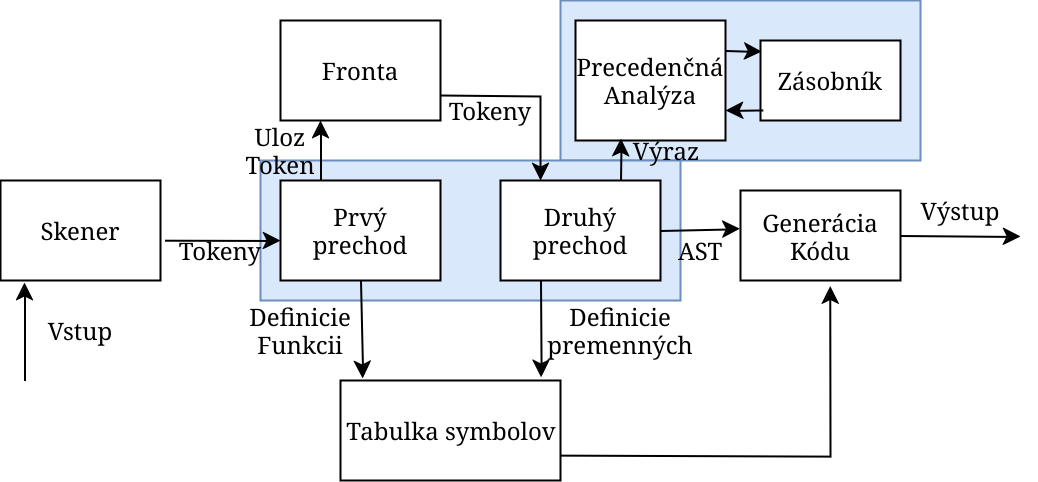
\includegraphics{Untitled Diagram.png}}
			\caption{Diagram komunikácie}
		\end{center}
	\end{figure}
	\subsection{Stručný popis}
	Parser (modrá časť diagramu) inicializuje všetky operácie v prekladači.  
	Preklad začína vložením programu v jazyku zig na
	 vstup. Skener (Na zavolanie) postupne fragmentuje vstup na jednotlivé lexémi a posiela ich vo forme tokenov do parseru.  Ako bolo už spomenuté, parser je dvojprechodový. Tokeny idú najprv cez prvý prechod, ktorý kontroluje syntax a sématiku iba pre hlavičky funkcií, ktoré následne ukladá do tabulky symbolov, aby informácie o nich boli dostupné v druhom prechode. Prvý prechod ukladá všetky prečítané tokeny do fronty. Z fronty si tokeny po jednom berie druhý prechod, ktorý kontroluje syntax a sématiku pre ostatok kódu. V prípade že v kóde sa nachádza výraz, zavolá sa precedenčná analýza, ktorá tento výraz pomocou zásobníka spracuje. Druhý prechod zároveň pridáva definované premenné do tabuľky symbolov  (samotnú tabuľku symbolov však aj využíva, napr. pre kontrolu redefinície).  Počas druhého prechodu sa zároveň vytvára ASS, ktorý po úspešnom dokončení analýzy slúži ako výstup a zároveň vstup do generátora kódu. Generátor kódu s pomocou tabuľky symbolou generuje cieľový kód.
	 	
	\newpage
	\section{Implementácia}
	\textbf{Skener: }\textit{lexer.*, token.h} (xhouzal00, xnemecp00)\\ 
	\textbf{Parser: }\textit{syntax.*, queue\_fill.*, precedence.*} (xluptas00, xklopam00)\\
	\textbf{Generátor kódu: }\textit{code\_gen.*} (xhouzal00, xnemecp00)\\
	\textbf{Hašovacia tabulka: }\textit{symtable.*} (xluptas00)\\
	\textbf{ASS: }\textit{tree.*} (xklopam00)\\
	\textbf{Zásobník: }\textit{stack.*} (xklopam00)\\
	\textbf{Fronta: }\textit{queue.*} (xluptas00)\\
	\textbf{Ostatné časti: }\textit{error.*} (xluptas00)\\
	\par Implementácia dátových štruktúr sa nachádza v jednotlitvých súboroch pomenovaných podľa danej štruktúry.
	\par Implementácia častí samotného prekladača spočíva v súboroch skenera, parsera, generátora a súboru \textit{error.*}, ktorý 
	implementuje základné pracovanie s chybami. Prvý prechod je implementovaný v súboroch \textit{queue\_fill.*} a druhý prechod je
	implementovaný v súboroch \textit{syntax.*}. \textit{syntax.c} zároveň obsahuje funkciu Main. Prílohy A, B, C, D ukazujú využitú teóriu, ktorá slúžila ako podklad pre jednotlivé časti prekladača.
	\subsection{Strom}
	\begin{wrapfigure}{l}{0.4\textwidth}
		\scalebox{0.25}{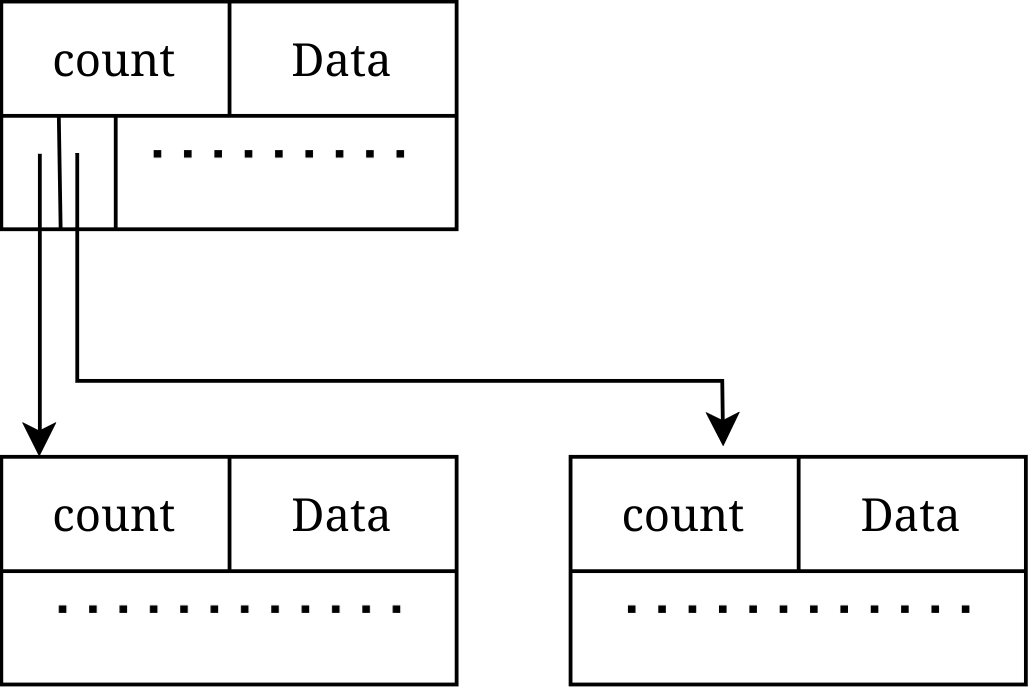
\includegraphics{Untitled Diagram(1).png}}
		\caption{Štruktúra stromu}
	\end{wrapfigure}
	Pre kompletnosť sme sa rozhodli vizualizovať ASS, ktorý sme navrhli pre tento prekladač.
	Ako je vidno na diagrame, tak každý uzol obsahuje 3 hlavné časti a to sú: \textit{count, data, children}, kde \textit{count}
	určuje počet detí, ktoré daný uzol má. Hlavná časť, \textit{data}, v sebe uchováva dáta potrebné na správne generovanie kódu
	(viac viď. tree.*). Posledná časť \textit{children} je pole ukazovaťelov na deti.  V texte ďalej ukážeme ako sa "kódujú" jednotlivé časti kódu do tohto stromu.
	\\\\
	\textbf{Typy uzlov} sú špecifikované v \textit{tree.h:15}. Strom má presne 1 koreň typu \textbf{ROOT\_NODE}  a má presne toľko detí, koľko je funkcií vo
	vstupnom programe. Tieto uzly sú typu \textbf{TOP\_FUNCTION\_NODE} a sú v nich uložené základné informácie o funkciách potrebné pre generáciu kódu.
	Z jednotlivých uzlov funkcií vychádzajú uzly špecifikujúce jednotlivé časti kódu. Tieto časti kódu sa delia na: \textit{priradenie, definíciu premennej, návrat, vetvenie, cyklus, volanie funkcie}. \\[0.6em]
	\textit{Priradenie} začína uzlom \textbf{ASSIGN\_NODE}, jeho prvé dieťa určuje do akej premennej sa priraďuje a jeho druhé dieťa určuje čo sa priraďuje (funkcia alebo výraz).\\[0.6em]
	\textit{Definícia premennej} má ten istý tvar ako \textit{priradenie} až na to, že vrchný uzol má typ \textbf{DEFINITION\_NODE}\\[0.6em]
	\textit{Návrat} začína uzlom typu \textbf{RETURN\_NODE} . Jeho jediným dieťaťom je strom výrazu, v prípade funkcie nevracajúcej hodnotu, nemá deti žiadne.\\[0.6em]
	\textit{Vetvenie} a \textit{cyklus} začínajú uzlom typu \textbf{WHILE\_NODE} alebo \textbf{IF\_NODE}. Na prvom mieste sa nachádza podmineka.  Nasleduje postupnosť častí kódu. Pokiaľ sa jedná o podmineku, začiatok druhej vetvy označuje dieťa typu \textbf{ELSE\_NODE} nasledovaná postupnosťou častí kódu.\\[0.6em]
	\textit{Volanie funkcie} začína uzlom \textbf{FUNCTION\_NODE} a jeho deti sú postupnosť argumentov. Podobne fungujú aj vstavané funkcie s miernou zmenou 
	typu hlavného uzla.\\[0.6em]
	\noindent Zaujímavým doplnkom stromu je inklúzia spätného odkazu na otca v každom uzle. Toto umožňuje celkom elegantné zanorovanie a vynorovanie v 
	rekurzívnom zostupe. Pokiaľ je napríklad volaná funkcia, program sa zanorí do uzlu \textbf{FUNCTION\_NODE} a zaplní ho uzlami argumentov. Po jeho spracovaní sa pomocou spätného odkazu program vynorí z tohto uzlu a je pripravený spracovať ďalšie riadky kódu.\\[0.6em]
	\noindent \textit{Generácia kódu} následne generuje kód jednoduchým prechádzaním tohto stromu.
	
	\subsection{Tabuľka symbolov}
		\begin{wrapfigure}{l}{0.35\textwidth}
			\scalebox{0.2}{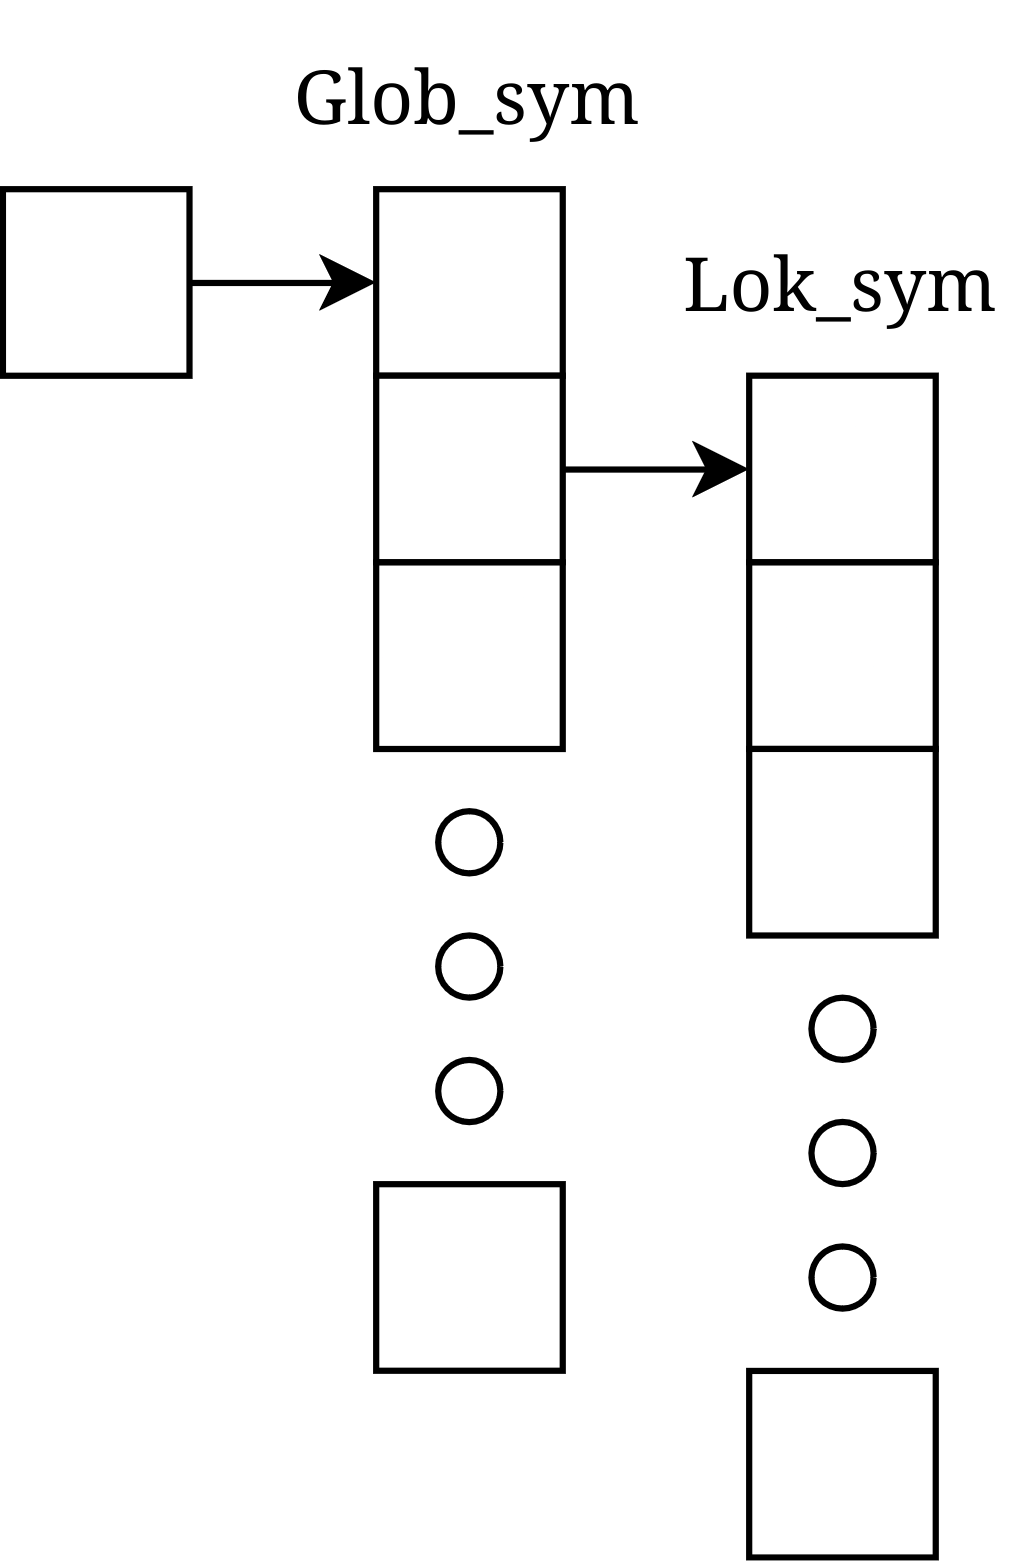
\includegraphics{diag.png}}
			\caption{Tabuľka symbolov}
		\end{wrapfigure}
	Tabuľku symbolov sme implementovali podľa zadania ako hašovaciu tabulku. V prekladači existuje ukazovaťeľ na \textit{globálnu tabuľku} v ktorej sú záznamy definovaných funkcií. Každá funkcia má v sebe odkaz na \textit{lokálnu tabuľku} symbolov.  Lokálna tabulka symbolov, obsahuje záznamy premenných v daných funkciách. Parametre funkcie sú na začiatku tiež interpretované ako lokálné premenné. Zaujímavosťou je určite riešenie rozsahu platnosti lokálnych premenných.
	 Namiesto riešenia zásobníka tabuliek symbolov sme vymysleli jednoduchý systém, kde každá premenná má svoj vlastný zásobník čísel. Tento zásobník určuje 
	 rozsah premennej následovne: premenné definované v tele hlavnej funkcie majú veľkosť zásobníku 1 a na zásobníku je číslica 1. Pokiaľ definujeme premennú v nejakom podbloku, na zásobník vložíme hodnotu, ktorá je jedinečná pre daný podblok (ilustrujeme obrázkom). Tabuľka je kvôli požadovanému implicitnému
	 zreťazeniu obmedzená na 1000 položiek, čo si uvedomujeme, že nie je najvhodnejšie riešiene, avšak veríme, že pre projekt bolo dostačujúce. 
	 \\
	\begin{figure}[ht]
		\begin{center}
			\scalebox{0.28}{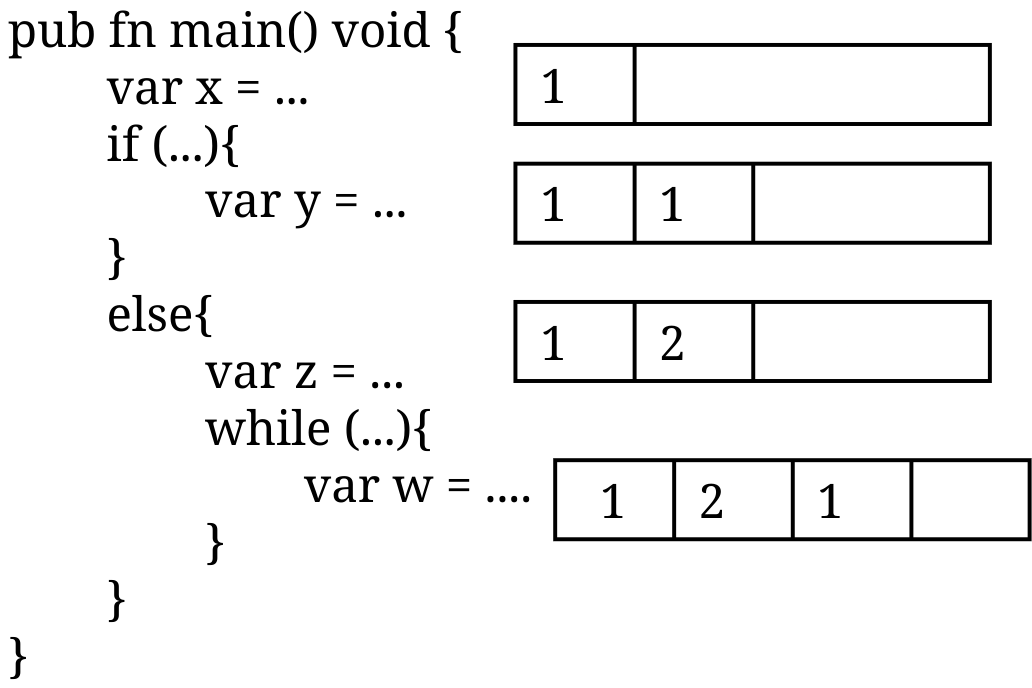
\includegraphics{sada.png}}
			\caption{Riešenie rozsahu platnosti}
		\end{center}
	\end{figure}
	\newpage

	\subsection{Implementácia ostatných častí}
	Ostatné časti (skener, parser, generácia kódu, zásobník, fronta) sú implementované štandardne metódami prednášanými na FIT VUT, preto ich špecifikáciu
	vynecháme.  
	
	\section{Práca v tíme}
	Na projekte sme pracovali počas celého semestra. Na správu verzií sme využívali platformu GitHub, ktorá nám umožnila prehľadnú organizáciu zdrojového kódu, sledovanie zmien a jednoduché riešenie prípadných konfliktov v kóde. Vďaka tomu mal každý člen tímu vždy prístup k aktuálnej verzii projektu. Na komunikáciu sme používali Discord, ktorý nám poskytol priestor na rýchlu výmenu informácií, plánovanie úloh a riešenie problémov v reálnom čase. Táto platforma bola užitočná najmä pri každodennom zdieľaní poznatkov alebo konzultáciách ohľadom implementácie jednotlivých častí projektu. Okrem online komunikácie sme sa raz týždenne stretávali osobne, aby sme spoločne zhodnotili doterajší pokrok, stanovili priority na nadchádzajúce obdobie a riešili zložitejšie časti projektu, ktoré si vyžadovali detailnú diskusiu. Tento pravidelný rytmus spolupráce zabezpečil plynulý vývoj projektu a pomohol nám efektívne rozdeliť prácu medzi jednotlivých členov tímu. Navyše sme sa rozdelili do tímov po dvoch podľa toho, ako sme ubytovaní na internátoch, čo nám umožnilo ešte rýchlejšiu komunikáciu pri problémoch špecifických pre jednotlivé tímy. Bodové rozdelenie odráža  čas vložený do projektu jednotlivými členmi tímu.
	
	\newpage
	\pagenumbering{gobble}
	\section{PRÍLOHA A - Konečný automat}
	\begin{figure}[ht]
		\begin{center}
			\scalebox{0.5}{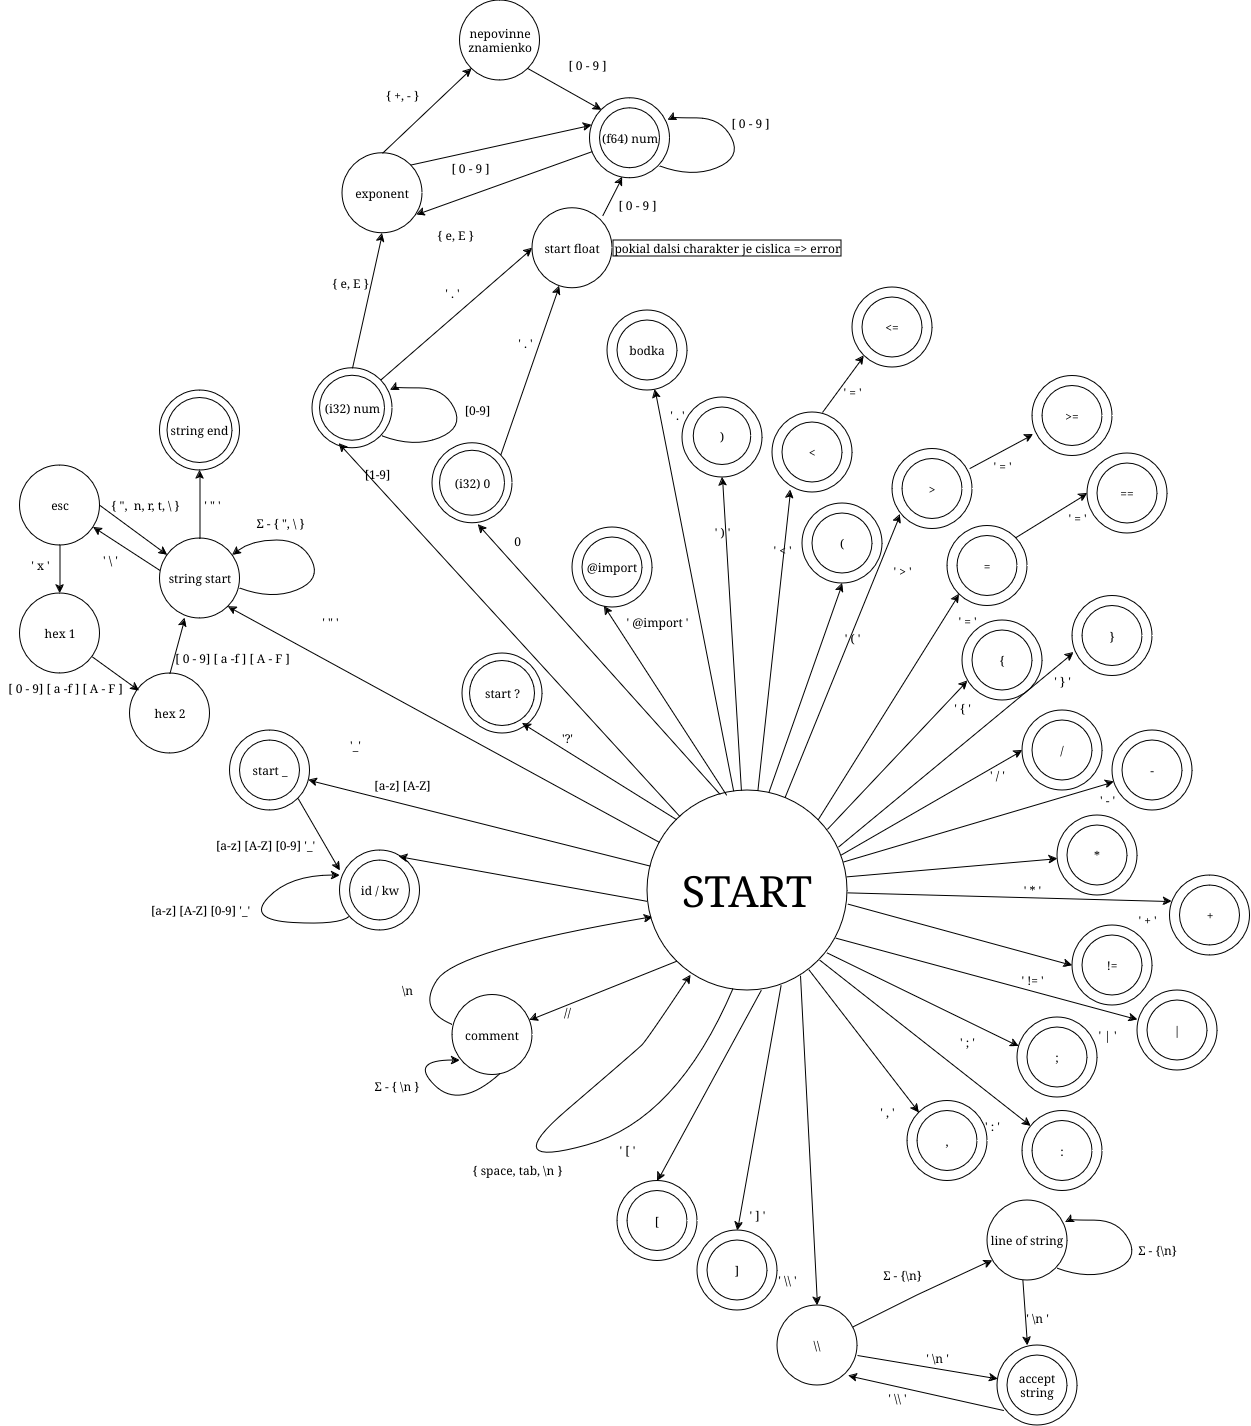
\includegraphics{xxx.png}}
		\end{center}
	\end{figure}
	
	\newpage
	\section{PRÍLOHA B - LL1 gramatika}
	<xxx> - xxx je neterminál\\
	'yyy' - yyy je terminál\\
	\\
	Pravidlá tokenov\\
	----------------------------------------------------------------------------------------------\\
	1. <ifj> -> 'IFJ'\\
	2. <at\_import> -> 'IMPORT'\\
	3. <eq> -> 'ASSIGN'\\
	4.<comma> -> 'COMMA'\\
	5. <colon> -> 'COLON'\\
	6. <op\_bracket> -> 'OPENING\_BRACKET'\\
	7. <cl\_bracket> -> 'CLOSING\_BRACKET'\\
	8. <op\_cr\_bracket> -> 'OPENING\_CURLY\_BRACKET'\\
	9. <cl\_cr\_bracket> -> 'CLOSING\_CURLY\_BRACKET'\\
	10. <op\_sq\_bracket> -> 'OPENING\_SQUARE\_BRACKET'\\
	11. <cl\_sq\_bracket> -> 'CLOSING\_SQUARE\_BRACKET'\\
	12. <string\_prolog> -> 'STRING' (tento string sa lisi od pravidla <string> tym ze musi nadobudat hodnotu ``ifj24.zig'')\\
	13. <semicolon> -> 'SEMICOLON'\\
	14. <pub> -> 'PUB'\\
	15. <fn> -> 'FN'\\
	16. <dot> -> 'DOT'\\
	17. <return> -> 'RETURN'\\
	18. <if> -> 'IF'\\
	19. <else> -> 'ELSE'\\
	20. <vertical\_bar> -> 'VERTICAL\_BAR'\\
	21. <while> -> 'WHILE'\\
	22. <eof> -> 'END\_OF\_FILE'\\
	23. <const> -> 'CONST'\\
	24. <var> -> 'VAR'\\
	25. <void> -> 'VOID'\\
	26. <type\_keyword> -> <op\_sq\_bracket> <cl\_sq\_bracket> 'U8'\\
	27. <type\_keyword> -> 'F64'\\
	28. <type\_keyword> -> 'I32'\\
	29. <string> -> 'STRING'\\
	30. <int> -> 'I32\_VAR'\\
	31. <float> -> 'F64\_VAR'\\
	32. <null> -> 'NULL\_VALUE'\\
	33. <id> -> 'ID'\\
	34. <id\_ifj> -> 'ID' (id.val sa musi zhodovat s nazvom neakej vstavanej funkcie)\\
	35. <underline> -> 'UNDERSCORE'\\
	36. <nullable> -> 'NULLABLE'\\
	37. <nullable> -> $\epsilon$\\
	\\
	Výrazi\\
	----------------------------------------------------------------------------------------------\\
	38. <var\_exp> -> <ifj\_call>\\
	39. <var\_exp> -> <fn\_call>\\
	40. <var\_exp> -> <exp> <semicolon>\\
	41. <null\_exp> -> <exp> <cl\_bracket>\\
	42. <null\_exp> -> <id> <cl\_bracket> <vertical\_bar> <id> <vertical\_bar> // zober 2 tokeny, pokial prvy je ID a druhy je cl\_bracket, vol tuto variantu, inak vol druhu\\
	43. <return\_exp> -> $\epsilon$\\
	44. <return\_exp> -> <exp>\\
	45. <exp> -> // call precedence analyzer\\
	\\
    Pomocné pravidlá\\
	----------------------------------------------------------------------------------------------\\
	46. <type> -> <nullable> <type\_keyword>\\
	47. <var\_const> -> <var>\\
	48. <var\_const> -> <const>\\
	49. <type\_fndef> -> <type>\\
	50. <type\_fndef> -> <void>\\
	51. <type\_vardef> -> <colon> <type>\\
	52. <type\_vardef> -> $\epsilon$\\
	53. <id\_assign> -> <underline>\\
	54. <id\_assing> -> <id>\\
	\\
	Hlavné previdlá\\
	----------------------------------------------------------------------------------------------\\
	55. <call\_params> -> $\epsilon$\\
	56. <call\_params> -> <string> <comma> <call\_params>\\
	57. <call\_params> -> <int> <comma> <call\_params>\\
	58. <call\_params> -> <float> <comma> <call\_params>\\
	59. <call\_params> -> <null> <comma> <call\_params>\\
	60. <call\_params> -> <id> <comma> <call\_params>\\
	61. <if\_while\_body> -> <op\_cr\_bracket> <fn\_body> <cl\_cr\_bracket>\\
	62. <var\_def> -> <var\_const> <id> <type\_vardef> <eq> <var\_exp>\\
	63. <assign> -> <id\_assign> <eq> <var\_exp>\\
	64. <fn\_call> -> <id> <op\_bracket> <call\_params> <cl\_bracket> <semicolon>\\
	65. <ifj\_call> -> <ifj> <dot> <ifj\_id> <op\_bracket> <call\_params> <cl\_bracket> <semicolon>\\
	66. <if\_else> -> <if> <op\_bracket> <null\_exp> <if\_while\_body> <else> <if\_while\_body>\\
	67. <cycle> -> <while> <op\_bracket> <null\_exp> <if\_while\_body>\\
	68. <fn\_return> -> <return> <return\_exp> <semicolon>\\
	69. <fn\_body> -> <var\_def> <fn\_body>\\
	70. <fn\_body> -> <assign> <fn\_body> // nahliadnutie do tabulky symbolov, pokial je ID variable, tak sa vola tato varianta\\
	71. <fn\_body> -> <fn\_call> <fn\_body> // nahliadnutie do tabulky symbolov, pokial je ID function alebo nedefinovane, tak sa vola tato varianta\\
	72. <fn\_body> -> <ifj\_call> <fn\_body> \\
	73. <fn\_body> -> <if\_else> <fn\_body>\\
	74. <fn\_body> -> <cycle> <fn\_body>\\
	75. <fn\_body> -> <fn\_return> <fn\_body>\\
	76. <fn\_body> -> $\epsilon$\\
	77. <params> -> <id> <colon> <type> <comma> <params>\\
	78. <params> -> $\epsilon$\\
	79. <fn\_def> -> <pub> <fn> <id> <op\_bracket> <params> <cl\_bracket> <type\_fndef> \\
	80. <functions> -> <fn\_def> <op\_cr\_bracket> <fn\_body> <cl\_cr\_bracket> <functions>\\
	81. <functions> -> <eof>\\
	82. <import\_def> -> <const> <ifj> <eq> <at\_import> <op\_bracket> <string\_prolog> <cl\_bracket> <semicolon>\\
	83. <start> -> <import\_def> <functions>
	\vfill
	\section{PRÍLOHA C - LL1 tabulka}
	\newpage
	\begin{figure}[ht]
		\begin{center}
			\scalebox{0.48}{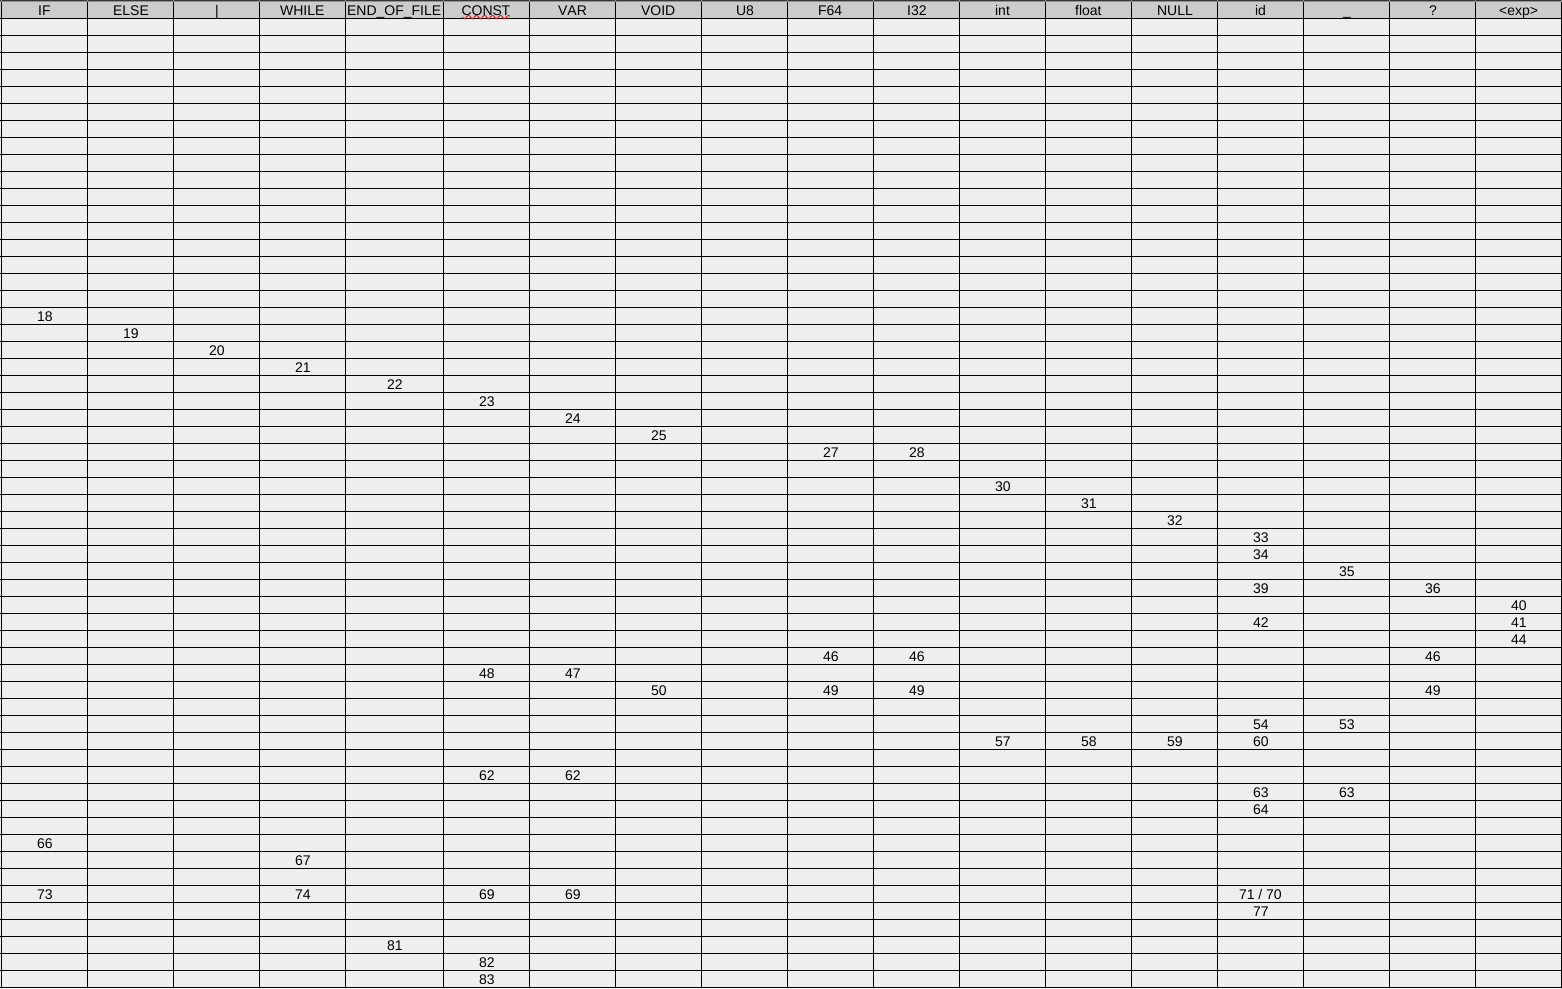
\includegraphics[angle=90]{LL222.png}}
		\end{center}
	\end{figure}
	\FloatBarrier
	\begin{figure}[ht]
		\begin{center}
			\scalebox{0.48}{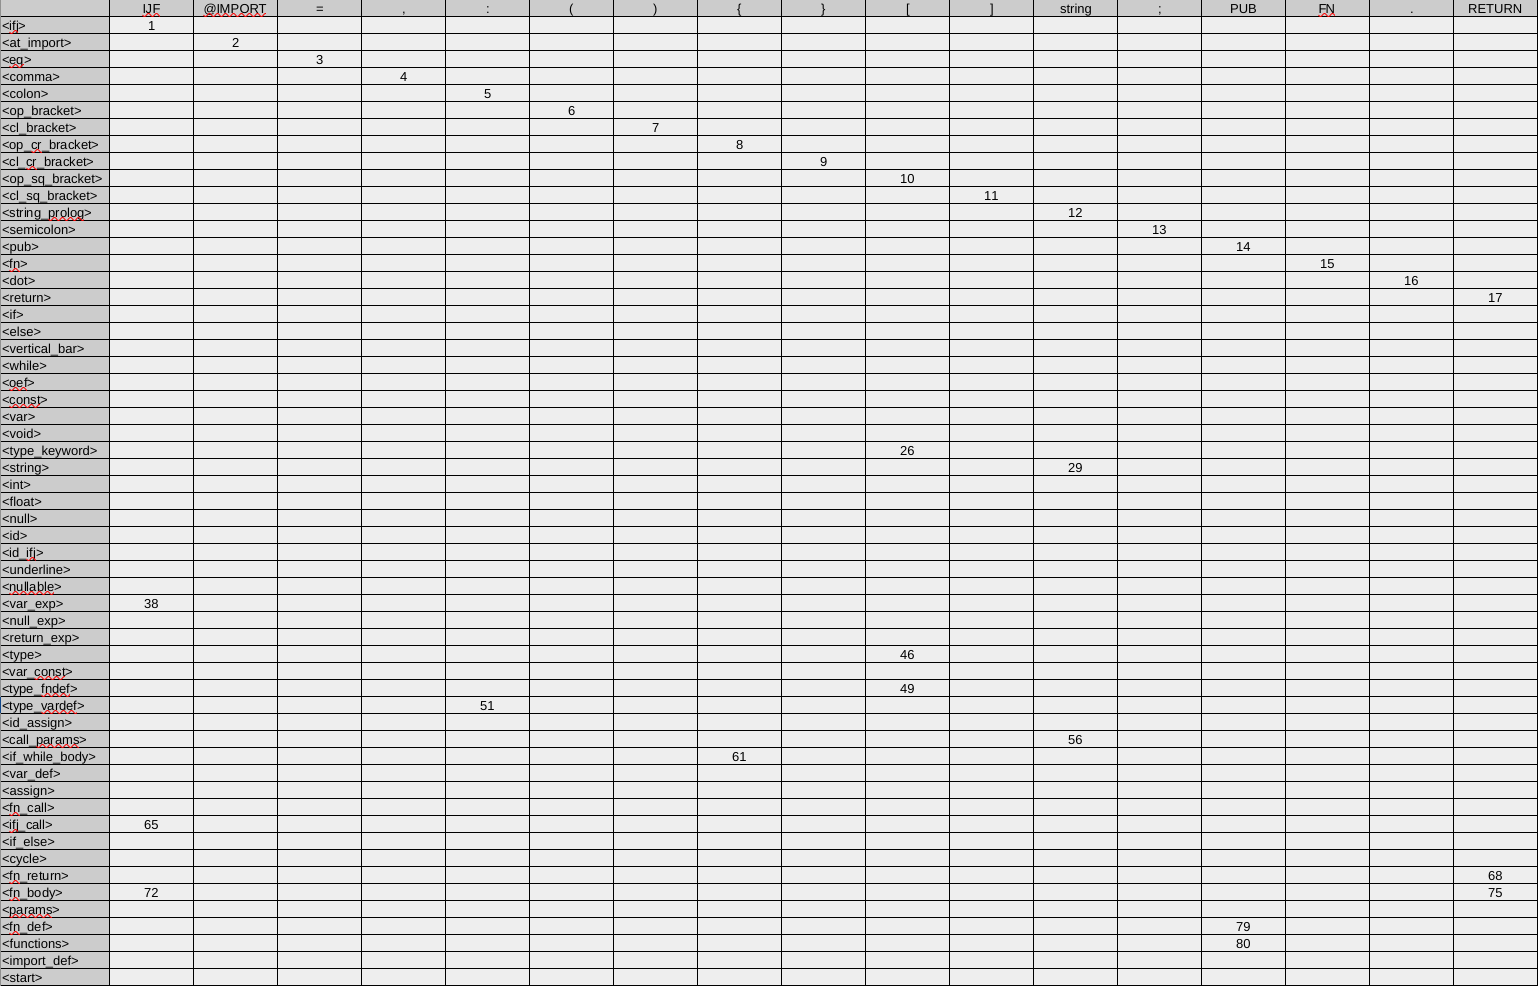
\includegraphics[angle=90]{LL11.png}}
		\end{center}
	\end{figure}
	\FloatBarrier
	
	\newpage
	\section{PRÍLOHA D - Precedenčná tabulka}
	\begin{figure}[ht]
		\begin{center}
			\scalebox{0.5}{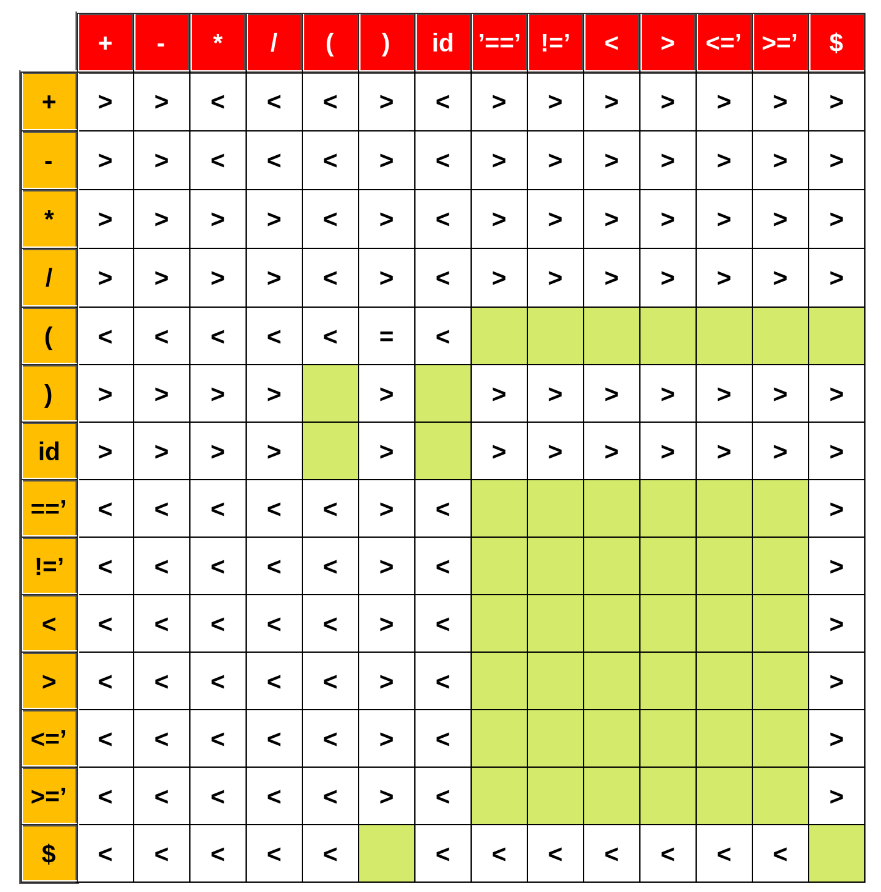
\includegraphics{asss.png}}
		\end{center}
	\end{figure}
	
\end{document}